\documentclass[11pt]{article}
\usepackage{fullpage}
\usepackage{times}
\usepackage{url}
\usepackage{color} % needed for todo
\usepackage{enumitem}
\usepackage{soul} % highlighting

\usepackage{graphicx} % Show images 
\usepackage{subcaption} % Show images side by side



\newcommand{\todo}[1]{\textcolor{cyan}{\textbf{[#1]}}}
\newcommand{\dan}[1]{\textcolor{blue}{{\it [Dan says: #1]}}}
\newcommand{\amit}[1]{\textcolor{red}{{\it [Amit: #1]}}}
\newcommand{\qi}[1]{\textcolor{green}{{\it [Qi: #1]}}}
\newcommand{\jeff}[1]{\textcolor{magenta}{{\it [Jeff: #1]}}}

\newcommand {\doublespace} {\addtolength{\baselineskip}{.5\baselineskip}}
\newcommand {\singlespace} {\addtolength{\baselineskip}{-.333\baselineskip}}

\begin{document}
%\pagestyle{empty}
\renewcommand{\thepage}{Facilities-\arabic{page}}
\setcounter{page}{1}

\def\myskip{3ex}

\centerline{\normalsize Rochester Institute of Technology}
\vspace{4 mm}
\centerline{\normalsize\bf Addressing Decision-Making Uncertainty in Cyber-physical Systems By Accounting for Tactic Volatility}


%\section*{Facilities}


\section*{Facilities Available to Accomplish Research Objectives}

% %\begin{figure}[h]
% \begin{wrapfigure}{R}{0.45\textwidth}
%  	\centering
%      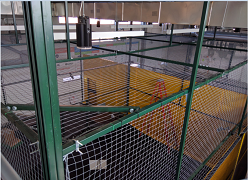
\includegraphics[scale=1.0]{images/SUFac1_sm.png}
%      \caption{UAV Cage Structure at Syracuse}
%      \label{fig:suUAVCage}
% \end{wrapfigure}
% %\end{figure}


We possess the necessary facilities to complete the proposed work. Research Computing\footnote{\url{http://rc.rit.edu/}} at RIT provides high performance computing resources (Figure~\ref{fig:RITResearchComputing}). Using a shared resource model, they have six Sun Fire X4600 M2 servers with eight quad-core 2.3GHz AMD processors and 64GB of memory each along with two Sun Fire X4500 servers that hold 48TB of raw data each. The Golisano College at RIT is comprised of five computing-oriented departments, with over 500 workstations. These workstations include Intel-based machines running Solaris, Windows, FreeBSD, or Linux; and other Apple, PC, and UNIX systems.


%The Center for Advanced Systems and Engineering (CASE) at Syracuse University, has an experienced and FAA-certified UAV pilot (Mr. Ian Joyce), supercomputing facilities, rapid prototyping and microprocessor boards for onboard testing of estimation and control algorithms. Co-PI Sanyal's home lab at the Syracuse Center of Excellence (CoE), which has a 20 ft × 20 ft × 18.5 ft indoor caged-in volume that is available for safe indoor testing of UAVs (Figure~\ref{fig:suUAVCage}). This indoor UAV lab posses several lightweight quadrotor UAVs; a DJI Phantom 4 quadrotor UAV; three custom-built UAVs; several LiDAR, optical and inertial sensors; two PX4 autopilots; BLDC motors with control units; and a customized autopilot with a sensor suite and onboard processor for autonomous navigation and control. It is mounted with an eight-camera Vicon motion capture system that can be used in two modes: (1) to provide motion estimation for feedback control of UAV platforms within the caged-in volume; and (2) as an external verification and validation system for onboard observer and control schemes for trajectory and target tracking. This camera system is accessed through a high-performance desktop computer that also acts as a control station to upload waypoints and Simulink-generated target code to UAVs flying inside the cage structure. %\hl{A picture of this space is given below left}, alongside a picture showing a still photo of an experiment using one of the Syma quadcopters in an autonomous trajectory following maneuver, where the motion feedback was provided by the Vicon system.

% \begin{figure}[h]
% \centering
% \begin{subfigure}{.5\textwidth}
%   \centering
%   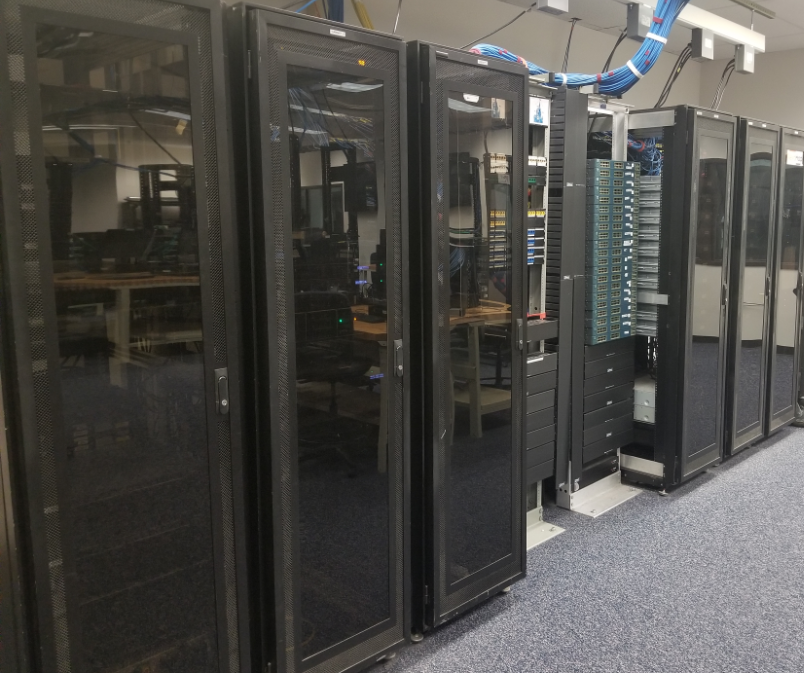
\includegraphics[scale=0.27]{images/CompLab2_sm.png}
%   \caption{Research Computing at RIT}
%   \label{fig:RITResearchComputing}
% \end{subfigure}%
% \begin{subfigure}{.5\textwidth}
%   \centering
%   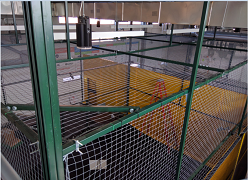
\includegraphics[scale=1.0]{images/SUFac1_sm.png}
%   \caption{UAV Cage Structure at Syracuse}
%   \label{fig:suUAVCage}
% \end{subfigure}
% \caption{Resources at RIT and Syracuse}
% \label{fig:Available Resources}
% \end{figure}


The National Technical Institute for the Deaf (NTID) is one of nine colleges at RIT and is the first and largest technical college in the world for Deaf/Hard-of-Hearing (Deaf/HoH) students. We will closely collaborate with NTID to recruit Deaf/Hard of Hearing students for the educational workshops. RIT also has ample resources to support the Deaf/Hard of Hearing workshop participants. 

RIT is home to numerous student groups including Women in Computing (WiC)\footnote{\url{http://wic.rit.edu/}}, the Society of Software Engineers (SSE)\footnote{\url{https://sse.rit.edu/}} and Women in Technology at RIT\footnote{\url{https://www.rit.edu/cast/wit/}}. We will work with these groups to hire underrepresented students whenever possible.


%The B. Thomas Golisano College of Computer and Information Sciences (GCCIS) at RIT provides technical support for developing and maintaining laboratory IT systems. The college is comprised of nine undergraduate seven graduate programs and one PhD programs. 



\begin{figure}[h]
%\begin{wrapfigure}{R}{0.45\textwidth}
 	\centering
 	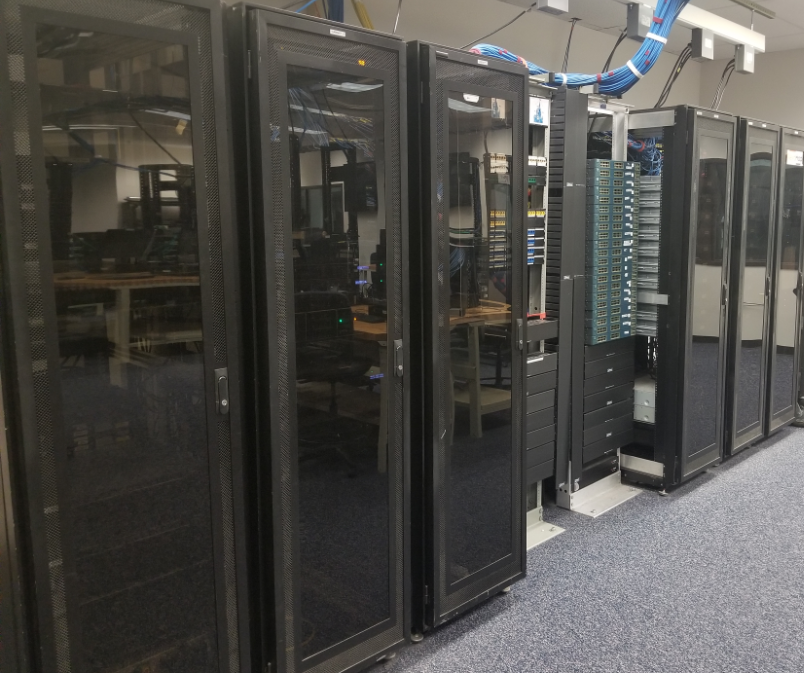
\includegraphics[scale=0.30]{images/CompLab2_sm.png}
   	\caption{Research Computing at RIT}
   	\label{fig:RITResearchComputing}
%\end{wrapfigure}
\end{figure}


% DK: Cut down if space is an issue



%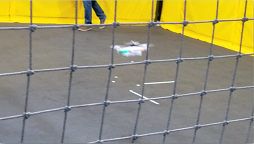
\includegraphics[scale=0.3]{images/SUFac2_sm.png} 

% \begin{figure}%
%     \centering
%     \subfloat[UAV Cage Structure St Syracuse]{{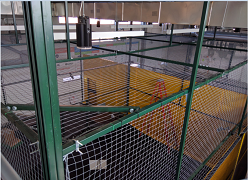
\includegraphics[scale=0.9]{images/SUFac1_sm.png} }}%
%     \qquad
%    \subfloat[label 2]{{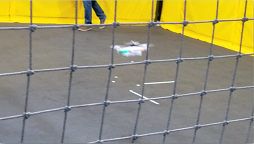
\includegraphics[scale=0.9]{images/SUFac2_sm.png} }}%
%     \caption{2 Figures side by side}%
%     \label{fig:Su}%
% \end{figure}











%RIT possesses a Guidance, Navigation and Controls (GN\&C) Laboratory and a state-of-the-art machine shop available to all students and faculty that can be used for constructing necessary any hardware as described in ``Goal XXX''. Algorithm development required for Goal X can be accomplished at RIT's GN\&C lab using currently owned algorithmic development tools such as Matlab. In addition, RIT possesses a unique outdoor netted UAV testing enclosure that can be used for final demonstration of the prototype flying UAV system. The advantage of the netted enclosure is no special FAA certificates or exemptions are required to perform outdoor demonstration testing. 





%\dan{Add in Syracuse info}
%\dan{Add in Griffis information}
%\dan{Add in several photos}

%RIT/Syracuse have the computers required for algorithmic development and demonstration tasks. We anticipate that no other capital equipment is required.



%% Tie each into tasks


% \bibliographystyle{abbrv}
% \bibliography{refs}


\end{document}
